\documentclass[a4paper, 12pt]{article}
% packages
\usepackage{amssymb}
\usepackage[fleqn]{mathtools}
\usepackage{tikz}
\usepackage{enumerate}
\usepackage{bussproofs}
\usepackage{xcolor}
\usepackage[margin=1.3cm]{geometry}
\usepackage{logicproof}
\usepackage{diagbox}
\usepackage{listings}
\usepackage{graphicx}
\usepackage{lstautogobble}
\usepackage{hyperref}
\usepackage{multirow}
\usetikzlibrary{arrows, shapes.gates.logic.US, circuits.logic.US, calc, automata, positioning}

% shorthand for verbatim
\catcode`~=\active
\def~#1~{\texttt{#1}}

% code listing
\lstdefinestyle{main}{
    numberstyle=\tiny,
    breaklines=true,
    showspaces=false,
    showstringspaces=false,
    tabsize=2,
    numbers=left,
    basicstyle=\ttfamily,
    columns=fixed,
    fontadjust=true,
    basewidth=0.5em,
    autogobble,
    xleftmargin=3.0ex,
    mathescape=true
}
\newcommand{\dollar}{\mbox{\textdollar}} %
\lstset{style=main}

% augmented matrix
\makeatletter
\renewcommand*\env@matrix[1][*\c@MaxMatrixCols c]{%
\hskip -\arraycolsep
\let\@ifnextchar\new@ifnextchar
\array{#1}}
\makeatother

% ceiling / floor
\DeclarePairedDelimiter{\ceil}{\lceil}{\rceil}
\DeclarePairedDelimiter{\floor}{\lfloor}{\rfloor}

% custom commands
\newcommand{\indefint}[2]{\int #1 \, \mathrm{d}#2}
\newcommand{\defint}[4]{\int_{#1}^{#2} #3 \, \mathrm{d}#4}
\newcommand{\dif}[2]{\frac{\mathrm{d}#1}{\mathrm{d}#2}}
\newcommand{\limit}[2]{\displaystyle{\lim_{#1 \to #2}}}
\newcommand{\summation}[3]{\sum\limits_{#1}^{#2} #3}
\newcommand{\intbracket}[3]{\left[#3\right]_{#1}^{#2}}
\newcommand{\ulsmash}[1]{\underline{\smash{#1}}}

\newcommand{\powerset}[0]{\wp}
\renewcommand{\emptyset}[0]{\varnothing}

\newcommand{\unaryproof}[2]{\AxiomC{#1} \UnaryInfC{#2} \DisplayProof}
\newcommand{\binaryproof}[3]{\AxiomC{#1} \AxiomC{#2} \BinaryInfC{#3} \DisplayProof}
\newcommand{\trinaryproof}[4]{\AxiomC{#1} \AxiomC{#2} \AxiomC{#3} \TrinaryInfC{#4} \DisplayProof}

% no indent
\setlength\parindent{0pt}

% reasoning proofs
\usepackage{ltablex}
\usepackage{environ}
\keepXColumns
\NewEnviron{reasoning}{
    \begin{tabularx}{\textwidth}{rlX}
        \BODY
    \end{tabularx}
}
\newcommand{\proofline}[3]{$(#1)$ & $#2$ & \hfill #3 \smallskip \\}
\newcommand{\proofarbitrary}[1]{& take arbitrary $#1$ \smallskip \\}
\newcommand{\prooftext}[1]{\multicolumn{3}{l}{#1} \smallskip \\}
\newcommand{\proofmath}[3]{$#1$ & = $#2$ & \hfill #3 \smallskip \\}
\newcommand{\prooftherefore}[1]{& $\therefore #1$ \smallskip \\}
\newcommand{\proofbc}[0]{\prooftext{\textbf{Base Case}}}
\newcommand{\proofis}[0]{\prooftext{\textbf{Inductive Step}}}

% reasoning er diagrams
\newcommand{\nattribute}[4]{
    \node[draw, state, inner sep=0cm, minimum size=0.2cm, label=#3:{#4}] (#1) at (#2) {};
}
\newcommand{\mattribute}[4]{
    \node[draw, state, accepting, inner sep=0cm, minimum size=0.2cm, label=#3:{#4}] (#1) at (#2) {};
}
\newcommand{\dattribute}[4]{
    \node[draw, state, dashed, inner sep=0cm, minimum size=0.2cm, label=#3:{#4}] (#1) at (#2) {};
}
\newcommand{\entity}[3]{
    \node[] (#1-c) at (#2) {#3};
    \node[inner sep=0cm] (#1-l) at ($(#1-c) + (-1, 0)$) {};
    \node[inner sep=0cm] (#1-r) at ($(#1-c) + (1, 0)$) {};
    \node[inner sep=0cm] (#1-u) at ($(#1-c) + (0, 0.5)$) {};
    \node[inner sep=0cm] (#1-d) at ($(#1-c) + (0, -0.5)$) {};
    \draw
    ($(#1-c) + (-1, 0.5)$) -- ($(#1-c) + (1, 0.5)$) -- ($(#1-c) + (1, -0.5)$) -- ($(#1-c) + (-1, -0.5)$) -- cycle;
}
\newcommand{\relationship}[3]{
    \node[] (#1-c) at (#2) {#3};
    \node[inner sep=0cm] (#1-l) at ($(#1-c) + (-1, 0)$) {};
    \node[inner sep=0cm] (#1-r) at ($(#1-c) + (1, 0)$) {};
    \node[inner sep=0cm] (#1-u) at ($(#1-c) + (0, 1)$) {};
    \node[inner sep=0cm] (#1-d) at ($(#1-c) + (0, -1)$) {};
    \draw
    ($(#1-c) + (-1, 0)$) -- ($(#1-c) + (0, 1)$) -- ($(#1-c) + (1, 0)$) -- ($(#1-c) + (0, -1)$) -- cycle;
}

% actual document
\begin{document}
    \section*{CO150 - Graphs and Algorithms}
        \subsection*{Prelude}
            The content discussed here is part of CO150 - Graphs and Algorithms (Computing MEng); taught by Iain Phillips, in Imperial College London during the academic year 2018/19. The notes are written for my personal use, and have no guarantee of being correct (although I hope it is, for my own sake). This should be used in conjunction with the notes.
        \subsection*{14th January 2019}
            Introduction to the structure of the course;
            \begin{enumerate}[{Part} I:]
                \itemsep0em
                \item Graphs
                \item Graph Algorithms
                \item Algorithm Analysis
                \item Introduction to Complexity
            \end{enumerate}
            An example graph with a real life application;
            \begin{center}
                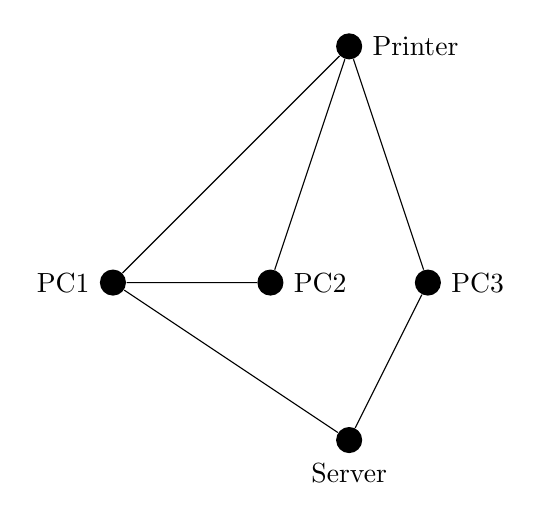
\begin{tikzpicture}
                    \node[circle, fill=black, label=right:PC2] (pc2) at (0, 0) {};
                    \node[circle, fill=black, label=left:PC1] (pc1) at (-2, 0) {};
                    \node[circle, fill=black, label=below:Server] (server) at (1, -2) {};
                    \node[circle, fill=black, label=right:PC3] (pc3) at (2, 0) {};
                    \node[circle, fill=black, label=right:Printer] (print) at (1, 3) {};

                    \draw
                    (print) -- (pc1)
                    (print) -- (pc2)
                    (print) -- (pc3)
                    (server) -- (pc1)
                    (server) -- (pc3)
                    (pc1) -- (pc2);
                \end{tikzpicture}
            \end{center}
            Note how all the PCs are directly connected to the printer, but PC2 can only reach the server through PC1. On the other hand, we can create a more general graph to display some features that may be less common;
            \begin{center}
                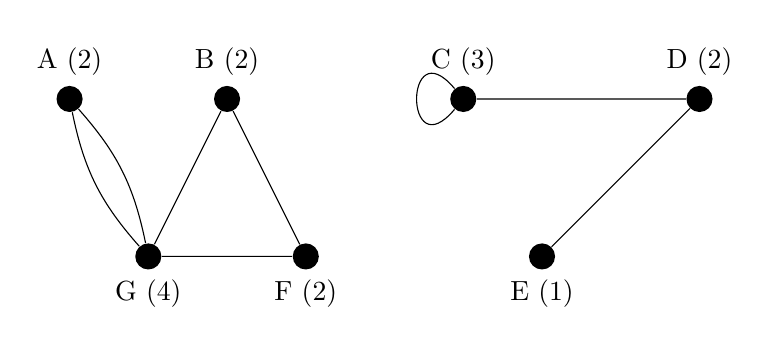
\begin{tikzpicture}
                    \node[circle, fill=black, label=above:A (2)] (a) at (0, 0) {};
                    \node[circle, fill=black, label=above:B (2)] (b) at (2, 0) {};
                    \node[circle, fill=black, label=above:C (3)] (c) at (5, 0) {};
                    \node[circle, fill=black, label=above:D (2)] (d) at (8, 0) {};
                    \node[circle, fill=black, label=below:E (1)] (e) at (6, -2) {};
                    \node[circle, fill=black, label=below:F (2)] (f) at (3, -2) {};
                    \node[circle, fill=black, label=below:G (4)] (g) at (1, -2) {};

                    \draw
                    (b) -- (g)
                    (g) -- (f)
                    (f) -- (b)
                    (c) -- (d)
                    (d) -- (e)
                    (a) edge[bend left=15] node{} (g)
                    (a) edge[bend right=15] node{} (g)
                    (c) edge[loop, out=230, in=130, distance=1cm] (c);
                \end{tikzpicture}
            \end{center}
            Note that this isn't actually two graphs; it's \textbf{disconnected components}. Between A, and G, there are two \textbf{parallel arcs / edges}, and C has \textbf{loop} with itself. I will continue to refer to this graph as the "example", for the remainder of this section, since it displays properties which we may want to analyse later.
            \medskip

            We can say that the left subgraph is robust, as it will remain connected against a single failure. However, the right subgraph isn't robust, as a failure between C, and D, or between E, and D would cause one of the nodes to become disconnected. We can then remedy this by adding a connection between C, and E.
            \medskip

            In the graph drawn above, the degrees are also specified - which is the number of arcs connected to it. Note that the degree of C is 3, as we count loops twice for consistency reasons. The sum of the degrees is 16, which is double the number of arcs (8). This is because each arc is counted twice (where it starts, and where it ends), therefore the sum of the degrees is always even. From that, we can then infer that the number of odd nodes (C, and E in our case) must be even. This is trivial to prove with arithmetic.
            \subsubsection*{Subgraphs}
                We can say that $G_1$ is a subgraph of $G_2$ if both of the following criteria apply;
                \begin{itemize}
                    \itemsep0em
                    \item $\text{nodes}(G_1) \subseteq \text{nodes}(G_2)$
                    \item $\text{arcs}(G_1) \subseteq \text{arcs}(G_2)$
                \end{itemize}
                A full (induced) subgraph occurs when we have a set of nodes, $X$, such that $X \subseteq \text{nodes}(G)$. Every connection between the nodes in $X$, that was present in $G$, exists in $G[X]$. Then $G^\prime$ is a full subgraph of $G$, if $G^\prime = G[X]$ for some $X$. For example, let $X = \{A, B, G\}$, from the example graph, then we have the following induced subgraph;
                \begin{center}
                    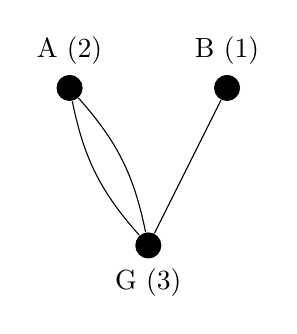
\begin{tikzpicture}
                        \node[circle, fill=black, label=above:A (2)] (a) at (0, 0) {};
                        \node[circle, fill=black, label=above:B (1)] (b) at (2, 0) {};
                        \node[circle, fill=black, label=below:G (3)] (g) at (1, -2) {};

                        \draw
                        (b) -- (g)
                        (a) edge[bend left=15] node{} (g)
                        (a) edge[bend right=15] node{} (g);
                    \end{tikzpicture}
                \end{center}
                If we have some subgraph $G^\prime$, and $\text{nodes}(G^\prime) = \text{nodes}(G)$, then it $G^\prime$ spans $G$.
            \subsubsection*{Adjacency Matrix}
                For the entry in the matrix $a_{i,j}$, it represents the number of arcs thast connect $i$ to $j$. In an undirected graph, this matrix is symmetric (such that $a^\top = a$). In our example, we're doing the rows, and columns, alphabetically. It's also important to note that we count each loop twice in a diagonal entry. We can determine the degree of a node by taking the sum of its respective row (or column), and find the number of arcs by taking the sum of all the values in the matrix, and then halving it.
                \begin{center}
                    $\begin{matrix}
                        \text{A} \\
                        \text{B} \\
                        \text{C} \\
                        \text{D} \\
                        \text{E} \\
                        \text{F} \\
                        \text{G}
                    \end{matrix}$$\begin{bmatrix}
                        0 & 0 & 0 & 0 & 0 & 0 & 2 \\
                        0 & 0 & 0 & 0 & 0 & 1 & 1 \\
                        0 & 0 & 2 & 1 & 0 & 0 & 0 \\
                        0 & 0 & 1 & 0 & 1 & 0 & 0 \\
                        0 & 0 & 0 & 1 & 0 & 0 & 0 \\
                        0 & 1 & 0 & 0 & 0 & 0 & 1 \\
                        2 & 1 & 0 & 0 & 0 & 1 & 0
                    \end{bmatrix}$
                \end{center}
            \subsubsection*{Adjacency Lists}
                You'll notice that in our graph, we have a lot of 0s, which makes it less efficient to store as an adjacency matrix; especially if we don't require random access to the degrees. We tend to use $n$ to represent the number of nodes (vertices), and $m$ to represent the number of arcs (edges). You'll note that the size of this is $\leq n + 2m$ (as we have $n$ nodes on the left, and each arc is counted twice, except for loops). Therefore, we can say a graph is sparse if $2m \ll n^2$. Since certain algorithms we work with only look at the arcs incident to a given node, a linked list will be better for sparse graphs.
                \begin{center}
                    \begin{tabular}{|c|@{ $\rightarrow$ }l|}
                        \hline
                        A & G, G \\
                        \hline
                        B & F, G \\
                        \hline
                        C & C, D \\
                        \hline
                        D & C, E \\
                        \hline
                        E & D \\
                        \hline
                        F & B, G \\
                        \hline
                        G & A, A, B, F \\
                        \hline
                    \end{tabular}
                \end{center}
            \subsubsection*{Big-Oh Notation}
                I'm too lazy to write out the example, but the idea is that we ignore constant factors, and only consider the most significant term; for example, we could summarise some algorithm that takes $3n^4 + 2n - 4631$ to run as $O(n^4)$. This has significant advantages, since it allows us to abstract away from the implementation / hardware specifics, and instead focus on the factors which determine growth.
            \subsubsection*{Isomorphism}
                In general, an isomorphism is a bijection that preserves connections. While the two graphs drawn below appear fairly different, they are isomorphic. Mapping from the left, to the right, we know that $3 \mapsto D$, simply because they are the only nodes with degree 2. It's also evident that $1 \mapsto B$, as it's the only node which has two sets of parallel arcs coming out of it. However, it doesn't matter which of 4, or 2, maps to $A$, or $C$. Therefore, we can say $4 \mapsto A, 2 \mapsto C$, or $4 \mapsto C, 2 \mapsto A$.
                \begin{center}
                    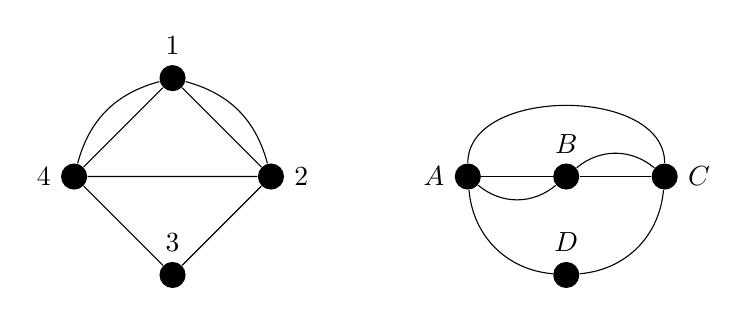
\begin{tikzpicture}[x=1.25cm, y=1.25cm]
                        \node[circle, fill=black, label=above:1] (1) at (0, 1) {};
                        \node[circle, fill=black, label=right:2] (2) at (1, 0) {};
                        \node[circle, fill=black, label=above:3] (3) at (0, -1) {};
                        \node[circle, fill=black, label=left:4] (4) at (-1, 0) {};
                        \draw
                        (4) -- (2)
                        (4) -- (1)
                        (4) -- (3)
                        (1) -- (2)
                        (2) -- (3)
                        (4) edge[bend left=30] (1)
                        (1) edge[bend left=30] (2);

                        \node[circle, fill=black, label=left:$A$] (A) at (3, 0) {};
                        \node[circle, fill=black, label=above:$B$] (B) at (4, 0) {};
                        \node[circle, fill=black, label=right:$C$] (C) at (5, 0) {};
                        \node[circle, fill=black, label=above:$D$] (D) at (4, -1) {};

                        \draw
                        (A) -- (B)
                        (B) -- (C)
                        (A) edge[bend left=90] (C)
                        (A) edge[bend right=40] (D)
                        (D) edge[bend right=40] (C)
                        (A) edge[bend right=40] (B)
                        (C) edge[bend right=40] (B);
                    \end{tikzpicture}
                \end{center}
                While we're able to check this fairly easily by simply looking at the graph, a computer would have to rearrange the LHS' adjacency matrix to the RHS' (or vice versa).
                \medskip

                Given two graphs, $G, G^\prime$, an isomorphism from $G$ to $G^\prime$ consists of two bijections (one-to-one mapping), as well as an additional restriction;
                \begin{itemize}
                    \itemsep0em
                    \item $f : \text{nodes}(G) \mapsto \text{nodes}(G^\prime)$
                    \item $g : \text{arcs}(G) \mapsto \text{arcs}(G^\prime)$
                    \item if $a \in \text{arcs}(G)$, with endpoints $n_1, n_2$, then the endpoints of $g(a)$ are $f(n_1), f(n_2)$ (see the diagram below for a visual example).
                \end{itemize}
                \begin{center}
                    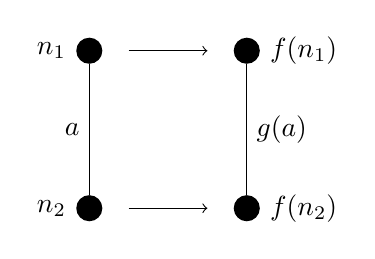
\begin{tikzpicture}
                        \node[circle, fill=black, label=left:$n_1$] (n1) at (0, 0) {};
                        \node[circle, fill=black, label=left:$n_2$] (n2) at (0, -2) {};
                        \node[circle, fill=black, label=right:$f(n_1)$] (fn1) at (2, 0) {};
                        \node[circle, fill=black, label=right:$f(n_2)$] (fn2) at (2, -2) {};
                        \draw
                        (n1) edge[left] node{$a$} (n2)
                        (fn1) edge[right] node{$g(a)$} (fn2)
                        ($(n1) + (0.5, 0)$) edge[->] ($(fn1) + (-0.5, 0)$)
                        ($(n2) + (0.5, 0)$) edge[->] ($(fn2) + (-0.5, 0)$);
                    \end{tikzpicture}
                \end{center}
                In order to confirm whether two graphs are isomorphic, the easiest approach is to first check the obvious; whether the number of arcs, nodes, and loops are the same, as well as the degrees of the nodes. If any of these are different, then the graphs cannot be isomorphic. However if they pass all the tests, then we can attempt to find a bijection on the nodes.
        \subsection*{17th January 2019}
            \subsubsection*{Complexity}
                Generally, the process of determining whether two graphs are isomorphic is computationally expensive, hence it has a high complexity. A naive approach would be to check all the permutations, which would then lead to a time complexity of $O(n!)$, which is worse than even exponential ($O(2^n)$).
            \subsubsection*{Automorphisms}
                An automorphism on $G$ is an isomorphism from $G$ to itself. Every graph has at least one automorphism (the identity). Consider the following graph;
                \begin{center}
                    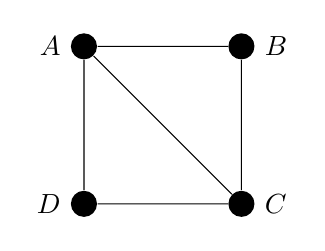
\begin{tikzpicture}
                        \node[circle, fill=black, label=left:$A$] (a) at (0, 0) {};
                        \node[circle, fill=black, label=right:$B$] (b) at (2, 0) {};
                        \node[circle, fill=black, label=right:$C$] (c) at (2, -2) {};
                        \node[circle, fill=black, label=left:$D$] (d) at (0, -2) {};
                        \draw
                        (a) -- (b) -- (c) -- (d) -- (a) -- (c);
                    \end{tikzpicture}
                \end{center}
                We can do the following method to find the number of automorphisms;
                \begin{itemize}
                    \itemsep0em
                    \item fix a node, $B$, it can go to where $D$ is, or stay (2 possibilities)
                    \item take the next node $A$, it can either stay where it is, or go to where $C$ is (2 possibilities), now fix it
                    \item take the next node $C$, it can only stay where it is, as it can't go to $D$ since $D$ isn't connected to $B$, nor does it have a degree of 3 (1 possibility), now fix it
                    \item finally $D$ can only stay where it is (1 possibility)
                    \item multiply all the possibilities, and we have 4 automorphisms
                \end{itemize}
            \subsubsection*{Planar Graphs}
                We can say a graph is planar if it can be drawn such that no arcs cross. Any non-planar graph contains $K_5$, or $K_{3,3}$ as a subgraph homeomorphic. We can say that two graphs are \textbf{homeomorphic} if they can be obtained by a series of operations such that an arc $x - y$, is replaced by two arcs $x - z$, and $z - y$. For example, the two graphs below are homeomorphic.
                \begin{center}
                    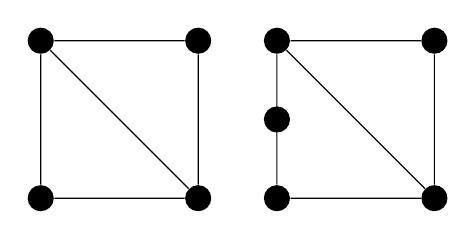
\begin{tikzpicture}
                        \node[circle, fill=black] (a) at (0, 0) {};
                        \node[circle, fill=black] (b) at (2, 0) {};
                        \node[circle, fill=black] (c) at (2, -2) {};
                        \node[circle, fill=black] (d) at (0, -2) {};
                        \draw
                        (a) -- (b) -- (c) -- (d) -- (a) -- (c);

                        \node[circle, fill=black] (a) at (3, 0) {};
                        \node[circle, fill=black] (b) at (5, 0) {};
                        \node[circle, fill=black] (c) at (5, -2) {};
                        \node[circle, fill=black] (d) at (3, -2) {};
                        \node[circle, fill=black] (e) at (3, -1) {};
                        \draw
                        (a) -- (b) -- (c) -- (d) -- (a) -- (c);
                    \end{tikzpicture}
                \end{center}
                There is a linear time algorithm to check whether a graph is planar; however in this case linear time means $O(n + m)$, with the previous definitions.
                \medskip

                Any planar graph splits the plane into regions, which are referred to as faces; the graph below splits it into 6 faces (including the outside region). With a graph $G$ that has $N$ nodes, $A$ arcs, and $F$ faces, Euler's formula states $F = A - N + 2$ for any connected planar graph.
                \begin{center}
                    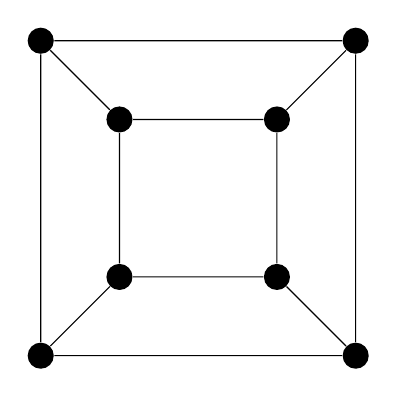
\begin{tikzpicture}
                        \node[circle, fill=black] (a) at (0, 0) {};
                        \node[circle, fill=black] (b) at (2, 0) {};
                        \node[circle, fill=black] (c) at (2, -2) {};
                        \node[circle, fill=black] (d) at (0, -2) {};
                        \node[circle, fill=black] (e) at (-1, 1) {};
                        \node[circle, fill=black] (f) at (3, 1) {};
                        \node[circle, fill=black] (g) at (3, -3) {};
                        \node[circle, fill=black] (h) at (-1, -3) {};
                        \draw
                        (a) -- (b) -- (c) -- (d) -- (a) -- (e) -- (f) -- (g) -- (h) -- (e)
                        (b) -- (f)
                        (c) -- (g)
                        (d) -- (h);
                    \end{tikzpicture}
                \end{center}
            \subsubsection*{Graph Colouring}
                Any (literal, real-life) map can be convereted into a simple planar graph by letting the countries represent nodes, and joining them if they are neighbours. This newly generated graph is known as the dual graph. We can say some graph $G$ is $k$-colourable, if the nodes of $G$ can be coloured with no more than $k$ colours, therefore every simple planar graph is 4-colourable.
            \subsubsection*{Bipartite Graphs}
                We can say a graph is bipartite if we can partition nodes($G$), into two sets $X$, and $Y$, such that no two nodes of $X$ are joined, and likewise for $Y$. A graph is biparite $\Leftrightarrow$ it is 2-colourable.
            \subsubsection*{Paths, and Connectedness}
                A path in a graph is a sequence of adjacent arcs, although normally described by the nodes that we pass through. A path is called \textbf{simple} if it doesn't repeat nodes, and a graph is \textbf{connected} if there is a path joining any two nodes.
                \medskip

                We can define a relation on nodes($G$) by $x \sim y \Leftrightarrow$ there is a path from $x$ to $y$. This is an equivalence relation, as we can prove it's reflexive, symmetric, and transitive.
                \begin{itemize}
                    \itemsep0em
                    \item $\forall x \in \text{nodes}(G) [x \sim x]$, $x$ is trivially connected to itself, hence it is reflexive
                    \item $\forall x,y \in \text{nodes}(G) [x \sim y \Rightarrow y \sim x]$, as we are working on an undirected graph, this follows trivially
                    \item $\forall x,y,z \in \text{nodes}(G) [x \sim y \land y \sim z \rightarrow x \sim z]$, follows trivially by definition of paths
                \end{itemize}
                A cycle (circuit) is a special type of path that finishes where it starts, has at least one arc, and doesn't reuse an arc. A graph which doesn't have cycles is \textbf{acyclic}.
        \subsection*{21st January 2019}
            \subsubsection*{Euler Paths / Circuits}
                An Euler path is a special type of path where each arc is used exactly once, and an Euler circuit is a cycle which uses each arc exactly once (therefore an EC is an EP which finishes at the start node). A connected graph has an EP $\Leftrightarrow$ there are 0, or 2 odd nodes, and there is an EC $\Leftrightarrow$ there are no odd nodes.
                \medskip

                We can justify it by saying that any intermediate node (ones which aren't the start node) have to be entered, and exited the same number of times (otherwise it wouldn't be an intermediate) node. Therefore, if 2 nodes of odd degree, then it follows that we start from one, and end on the other.
                \medskip

                Consider the following nodes; $n$, $n^\prime$ being the start, and end (the odd nodes of the path), and arbitrary intermediate nodes $i$. Start at $n$, and keep going until we can go no further ($n^\prime$). If we've stopped at $n$, then there must be a spare arc, as we've started, and 'ended' at an odd node. If we stop at some arbitrary $i \neq n^\prime$, then we've still got more arcs, since $i$ is even.
            \subsubsection*{Hamiltonian Path / Circuits}
                A Hamiltonian path is one that visits each node exactly once, and similarly a Hamiltonian circuit returns to the start node. For this, we will only consider simple graphs, since we won't ever follow a loop, or a parallel arc. In order for there to be a HP, we need a connected graph, and for a HC to exist, each node must have a degree $\geq 2$. To determine whether a circuit exists, we can take a brute force approach, since a circuit is really just a permutation on the set of nodes; such that for $n$ nodes, we have $\pi : \{1, ..., n\} \mapsto \{1, ..., n\}$. However, for this to be a circuit, we need $\pi(i)$ to be adjacent to $\pi(i + 1)$, and so on. As we have $n!$ possible circuits, this is far too slow. There exists a dynamic programming approach that reduces this to $O(n^22^n)$, but that is still exponential. Compared to EPP, which has $O(n^2)$ time. HCP has been shown to be NP-complete, and are therefore not solvable in polynomial time.
            \subsubsection*{Trees}
                A tree is an acyclic connected graph (whether we specify it's rooted, or nonrooted, depends on the author). The root of $G$ is a distinguished node. Assuming a rooted graph, the depth of a node $x$ is the distance along the unique path from the root to $x$. If $x$ isn't the root node, the parent of $x$ is the node directly before it in the path from the root to $x$. The depth of tree is the maximum of the depths of all its nodes.
                \medskip

                A spanning tree of a graph $G$, is a tree, $T$, such that $\text{nodes}(T) = \text{nodes}(G)$, and $\text{arcs}(T) \subseteq \text{arcs}(G)$. The spanning trees are not necessarily unique.
            \subsubsection*{Directed Graphs}
                While we generally cover undirected graphs in this course, it makes sense in some applications for the arcs to be directed. For each $a \in \text{arcs}(G)$, it is associated with an \textbf{ordered} pair of nodes. In diagrams, these are shown with arrows. In a path for $a_1, ..., a_n$, the source of $a_{i + 1}$, must match the target of $a_i$. We define the indegree as the number of arcs entering, and likewise the outdegree is the number of args leaving. For any directed graph, the sum of the indegree of all nodes, and the outdegree of all nodes is equal to the number of arcs. We say a directed graph is strongly connected if there exists a path between any two nodes in $G$.
        \subsection*{24th January 2019}
            \subsubsection*{Tree Traversal Algorithms}
                The two types of traversal covered in this course are depth-first search (DFS), and breadth-first search (BFS). While they are similar in many ways, they also have quite a few differences.
                \medskip

                In depth first search, we choose one of the adjacent nodes to the start; from there, we then spawn another depth first search. This is done recursively until there aren't any more (unvisited) adjacent nodes. At this point, the spawned DFS returns back to the parent node, where it checks the next adjacent node (normally ordered by how the adjaceny list / matrix is stored). It does this until we have visited all of the nodes, and then returns back all the way to the start.
                \medskip

                In contrast to DFS, breadth-first search goes through all the adjacent nodes, and then goes deeper. This means that we only check the nodes adjacent to the ones adjacent to the start node, after all of the nodes directly adjacent to the start node have been visited.
                \medskip

                You'll note that the distance between 1, and 8, is 5 in DFS, but only 1 in BFS. In BFS, the depth of any node is its distance from the start. However, both generate spanning trees on $G$.
                \begin{center}
                    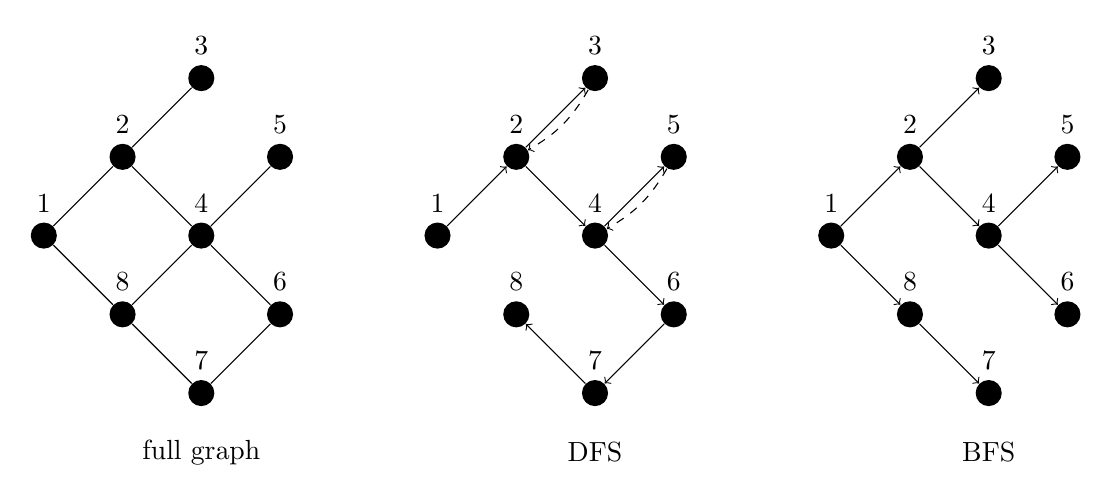
\begin{tikzpicture}
                        \node[] () at (2, -2.75) {full graph};
                        \node[] () at (7, -2.75) {DFS};
                        \node[] () at (12, -2.75) {BFS};
                        \foreach \x in {0, 1, 2} {
                            \node[circle, fill=black, label=above:1] (1-\x) at (5*\x, 0) {};
                            \node[circle, fill=black, label=above:2] (2-\x) at (1 + 5*\x, 1) {};
                            \node[circle, fill=black, label=above:3] (3-\x) at (2 + 5*\x, 2) {};
                            \node[circle, fill=black, label=above:4] (4-\x) at (2 + 5*\x, 0) {};
                            \node[circle, fill=black, label=above:5] (5-\x) at (3 + 5*\x, 1) {};
                            \node[circle, fill=black, label=above:6] (6-\x) at (3 + 5*\x, -1) {};
                            \node[circle, fill=black, label=above:7] (7-\x) at (2 + 5*\x, -2) {};
                            \node[circle, fill=black, label=above:8] (8-\x) at (1 + 5*\x, -1) {};
                        }
                        \draw
                        (1-0) -- (2-0) -- (3-0)
                        (1-0) -- (8-0) -- (7-0) -- (6-0) -- (4-0) -- (5-0)
                        (8-0) -- (4-0) -- (2-0);

                        \draw
                        (1-1) edge[->] (2-1)
                        (2-1) edge[->] (3-1)
                        (3-1) edge[bend left=15, ->, dashed] (2-1)
                        (2-1) edge[->] (4-1)
                        (4-1) edge[->] (5-1)
                        (5-1) edge[bend left=15, ->, dashed] (4-1)
                        (4-1) edge[->] (6-1)
                        (6-1) edge[->] (7-1)
                        (7-1) edge[->] (8-1);

                        \draw
                        (1-2) edge[->] (2-2)
                        (1-2) edge[->] (8-2)
                        (2-2) edge[->] (3-2)
                        (2-2) edge[->] (4-2)
                        (8-2) edge[->] (7-2)
                        (4-2) edge[->] (5-2)
                        (4-2) edge[->] (6-2);
                    \end{tikzpicture}
                \end{center}
                In order to formalise this, let us consider the graph to be traversed as an adjaceny list, a boolean array of nodes (which are visited), and the parent is the parent node in the search tree. The output will be the nodes visited in order.
                \begin{lstlisting}
                    procedure dfs(x):
                      visited[x] = true
                      print x
                      for y in adj[x]:
                        if not visited[y]:
                          parent[y] = x;
                          dfs(y)
                          # at this point, control is returned to x
                          # we don't need the parent in this case, but other applications may use it
                \end{lstlisting}
                The running time of DFS is $O(n + m)$, therefore it's linear. However, this implementation may have some overhead due to recursion.
                \begin{lstlisting}
                    procedure bfs(x):
                      visited[x] = true
                      print[x]
                      enqueue(x, Q)
                      while not isempty(Q):
                        y = front(Q)
                        for z in adj[y]:
                          if not visited[z]:
                            visited[z] = true
                            print z
                            parent[z] = y
                            enqueue(z, Q)
                        dequeue(Q)
                \end{lstlisting}
                The size of the queue represents the breadth of the front. Once again, the time complexity is $O(n + m)$.
            \subsubsection*{Applications of Traversal}
                The algorithms used above also work on non-connected graphs. If we analyse the set of visited nodes, and see that it isn't the same as the set of all nodes, then it is clear that the graph is not connected. As such, we have an $O(n + m)$ algorithm for detecting non-connected graphs.
                \medskip

                We can trivially say that a graph has a cycle if it has $\geq n$ arcs. Alternatively, we can use DFS; if we encounter a node that has already been visited (other than by backtracking), then it has a cycle.
                \medskip

                It's also trivial to modify BFS to find the distance of each node, by having a running counter. Due to how BFS is implemented, we can also extract the shortest path from ~y~; as ~y, parent[y], parent[parent[y]], ..., start~.
            \subsubsection*{Weihted Graphs}
                We can associate a cost with each arc on a network. We can define a weighted graph as a graph, $G$, with a weight function $W : \text{arcs}(G) \mapsto \mathbb{R}^+$. With weights, we're able to consider the following problems; finding an MST (minimum spanning tree), finding shortest paths, and finding a shortest circuit.
                \medskip

                We're only going to consider simple graphs, as there is no point in taking a loop if we're trying to minimise cost, nor is there any point in taking the more expensive arc in a parallel arc.
            \subsubsection*{MST Algorithms}
                We can say that $T$ is a minimum spanning tree for $G$m if $T$ is a spanning tree for $G$, and no other spanning tree for $G$ has a smaller weight. Once again, MSTs do not have to be unique.
                \medskip

                The main idea in Prim's algorithm is to add the shortest arc that will extend the tree. This is an example of a greedy algorithm, which gives a short-term advantage byt may not be the best overall (it is in this case). At any stage in Prim's algorithm, we have three types of nodes; tree nodes (which are already part of the MST), candidate nodes - which are fringe nodes adjacent to a tree node, and the rest are unseen nodes. At the start, all nodes are unseen.
                \begin{center}
                    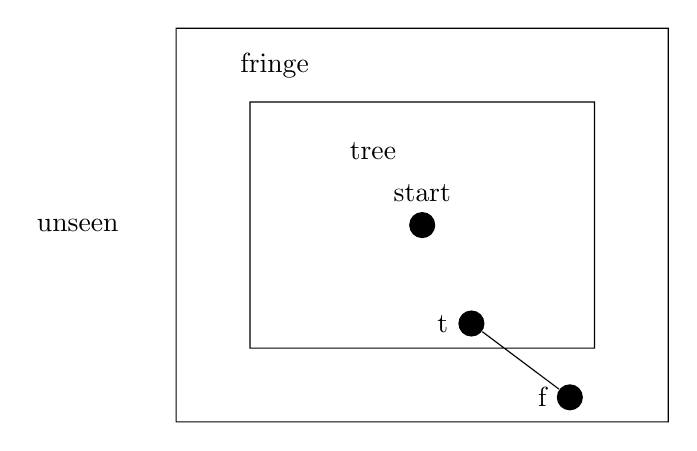
\begin{tikzpicture}[x=1.25cm, y=1.25cm]
                        \node[circle, fill=black, label=above:start] () at (2.5, -2) {};
                        \node[circle, fill=black, label=left:t] (t) at (3, -3) {};
                        \node[circle, fill=black, label=left:f] (f) at (4, -3.75) {};
                        \node[] () at (1, -0.375) {fringe};
                        \node[] () at (2, -1.25) {tree};
                        \node[] () at (-1, -2) {unseen};
                        \draw
                        (0, 0) -- (5, 0) -- (5, -4) -- (0, -4) -- cycle
                        (0.75, -0.75) -- (4.25, -0.75) -- (4.25, -3.25) -- (0.75, -3.25) -- cycle
                        (t) -- (f);
                    \end{tikzpicture}
                \end{center}
                The general idea is to pick a random node (doesn't matter which, as all nodes will be in the MST by definition)
\end{document}
